%%%%%%%%%%%%  Generated using docx2latex.com  %%%%%%%%%%%%%%

%%%%%%%%%%%%  v2.0.0-beta  %%%%%%%%%%%%%%

\documentclass[12pt]{article}
\usepackage{amsmath}
\usepackage{latexsym}
\usepackage{amsfonts}
\usepackage[normalem]{ulem}
\usepackage{array}
\usepackage{amssymb}
\usepackage{graphicx}
\usepackage[backend=biber,
style=numeric,
sorting=none,
isbn=false,
doi=false,
url=false,
]{biblatex}\addbibresource{bibliography.bib}

\usepackage{subfig}
\usepackage{wrapfig}
\usepackage{wasysym}
\usepackage{enumitem}
\usepackage{adjustbox}
\usepackage{ragged2e}
\usepackage[svgnames,table]{xcolor}
\usepackage{tikz}
\usepackage{longtable}
\usepackage{changepage}
\usepackage{setspace}
\usepackage{hhline}
\usepackage{multicol}
\usepackage{tabto}
\usepackage{float}
\usepackage{multirow}
\usepackage{makecell}
\usepackage{fancyhdr}
\usepackage[toc,page]{appendix}
\usepackage[hidelinks]{hyperref}
\usetikzlibrary{shapes.symbols,shapes.geometric,shadows,arrows.meta}
\tikzset{>={Latex[width=1.5mm,length=2mm]}}
\usepackage{flowchart}\usepackage[paperheight=11.0in,paperwidth=8.5in,left=1.0in,right=1.0in,top=1.0in,bottom=1.0in,headheight=1in]{geometry}
\usepackage[utf8]{inputenc}
\usepackage[T1]{fontenc}
\TabPositions{0.5in,1.0in,1.5in,2.0in,2.5in,3.0in,3.5in,4.0in,4.5in,5.0in,5.5in,6.0in,}

\urlstyle{same}


 %%%%%%%%%%%%  Set Depths for Sections  %%%%%%%%%%%%%%

% 1) Section
% 1.1) SubSection
% 1.1.1) SubSubSection
% 1.1.1.1) Paragraph
% 1.1.1.1.1) Subparagraph


\setcounter{tocdepth}{5}
\setcounter{secnumdepth}{5}


 %%%%%%%%%%%%  Set Depths for Nested Lists created by \begin{enumerate}  %%%%%%%%%%%%%%


\setlistdepth{9}
\renewlist{enumerate}{enumerate}{9}
		\setlist[enumerate,1]{label=\arabic*)}
		\setlist[enumerate,2]{label=\alph*)}
		\setlist[enumerate,3]{label=(\roman*)}
		\setlist[enumerate,4]{label=(\arabic*)}
		\setlist[enumerate,5]{label=(\Alph*)}
		\setlist[enumerate,6]{label=(\Roman*)}
		\setlist[enumerate,7]{label=\arabic*}
		\setlist[enumerate,8]{label=\alph*}
		\setlist[enumerate,9]{label=\roman*}

\renewlist{itemize}{itemize}{9}
		\setlist[itemize]{label=$\cdot$}
		\setlist[itemize,1]{label=\textbullet}
		\setlist[itemize,2]{label=$\circ$}
		\setlist[itemize,3]{label=$\ast$}
		\setlist[itemize,4]{label=$\dagger$}
		\setlist[itemize,5]{label=$\triangleright$}
		\setlist[itemize,6]{label=$\bigstar$}
		\setlist[itemize,7]{label=$\blacklozenge$}
		\setlist[itemize,8]{label=$\prime$}

\setlength{\topsep}{0pt}\setlength{\parindent}{0pt}

 %%%%%%%%%%%%  This sets linespacing (verticle gap between Lines) Default=1 %%%%%%%%%%%%%%


\renewcommand{\arraystretch}{1.3}


%%%%%%%%%%%%%%%%%%%% Document code starts here %%%%%%%%%%%%%%%%%%%%



\begin{document}
{\fontsize{24pt}{28.8pt}\selectfont \textbf{\textcolor[HTML]{0C343D}{\uline{Skewed Associative Cache}}}\par}\par


\vspace{\baselineskip}
{\fontsize{14pt}{16.8pt}\selectfont There goes an inherent trade-off between direct mapped cache and N-way set associative cache in terms of hit rate and time required to access a given memory address. Direct mapped cache has a fast access to a given address but at the same time, due to allocation of only a single block to a given address in the whole cache, it has a low hit rate. On the other hand, set associative cache has to search in at most N-blocks while searching for a given address which makes it a little bit slow, but since a given memory address can now be put into N different blocks, it has a high hit rate.\par}\par


\vspace{\baselineskip}
{\fontsize{14pt}{16.8pt}\selectfont Now here comes yet another type of cache, the Skewed associative cache. It has almost the same hardware implementation as that of a set associative cache but is twice as faster than a set associative cache.\par}\par


\vspace{\baselineskip}

\vspace{\baselineskip}

\vspace{\baselineskip}

\vspace{\baselineskip}
{\fontsize{24pt}{28.8pt}\selectfont \textbf{\textcolor[HTML]{0C343D}{\uline{So how is it exactly different from Set Associative Cache ?}}}\par}\par


\vspace{\baselineskip}
{\fontsize{14pt}{16.8pt}\selectfont A Set Associative Cache and a Skewed Associative cache are both multi bank cache. A multi bank cache is one which has more than one block allocated for a given memory address. If a particular address of main memory can be allocated to N blocks in the cache, then the cache is said to have N banks. That memory address can then go to any of these N banks depending upon the replacement policy used in putting the new memory address.\par}\par


\vspace{\baselineskip}
{\fontsize{14pt}{16.8pt}\selectfont The way in which Skewed and Set associative cache differ from each other is in the way of allocation of block in these different banks. The set associative cache uses the same function to allocate block in different banks. A case for 2-way set associative cache (having 2 different banks) can be illustrated from the following figure.\par}\par



%%%%%%%%%%%%%%%%%%%% Figure/Image No: 1 starts here %%%%%%%%%%%%%%%%%%%%

\begin{figure}[H]
	\begin{Center}
		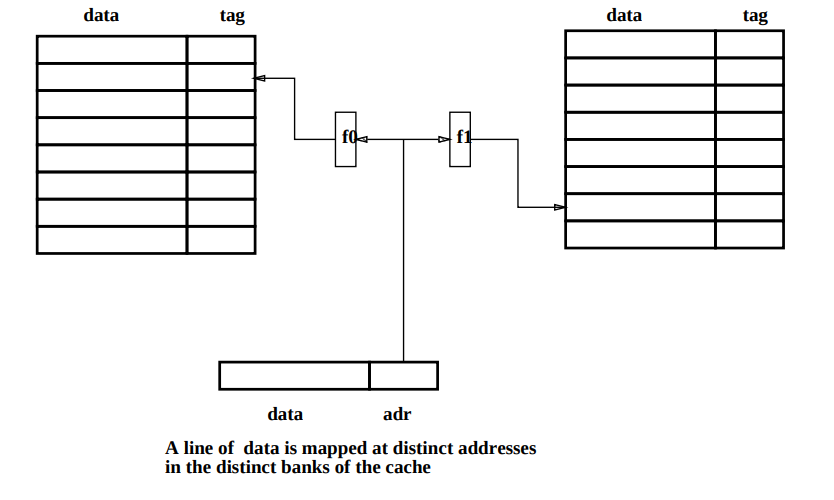
\includegraphics[width=6.5in,height=3.97in]{./media/image1.png}
	\end{Center}
\end{figure}


%%%%%%%%%%%%%%%%%%%% Figure/Image No: 1 Ends here %%%%%%%%%%%%%%%%%%%%

\par


\vspace{\baselineskip}

\vspace{\baselineskip}

\vspace{\baselineskip}
{\fontsize{14pt}{16.8pt}\selectfont Here the same function (say f) is used to map a given memory address to a block in different banks. The block chosen finally depends upon the replacement policy used.\par}\par


\vspace{\baselineskip}
{\fontsize{14pt}{16.8pt}\selectfont On the other hand, a N-way Skewed Associative cache also has N banks, but the block assignment in these banks is done by different functions (say f1 and f2). \par}\par


\vspace{\baselineskip}

\vspace{\baselineskip}

\vspace{\baselineskip}

\vspace{\baselineskip}

\vspace{\baselineskip}

\printbibliography
\end{document}